%!TEX root = /Users/oroce/Documents/msc-szakdolgozat/dolgozat.tex
A folyamatos integrációnál mivel naponta több verzió is kikerülhet, sőt párhuzamosan akár több csapat vagy fejlesztő is a produkciós rendszerbe helyezhet át funkciókat, ezért nagyon fontos, hogy a rendszer folyamatosan tájékoztassa a csapatokat az élesített és elkészített funkciók működéséről, hibáiról illetve a többi szereplő által fejlesztett funkciók állapotáról. Mindehhez két dologra van szükség: a kommunikációra és a rendszer minden apró részének monitorozására, mert ezáltal a hibák gyorsan kiszűrhetőek, a reakció idő csökkenthető és mindenki valós időben láthatja, hogy mi történik a rendszerben, azaz transzparens lesz, amelynek köszönhetően a szervezetnek könnyebb a részegységek megismerése, felelősségi köreik meghatározása.

\section{Chat rendszer}
A fejlesztői csapatok illetve a csapattagok közti kommunikáció rendkívül fontos, mely persze történhet verbálisan, azonban ez megszakíthatja a munkát, illetve távoli munkavégzés esetén (főleg ha a résztvevők más országból végzik a munkát) akkor sokkal jobb megoldás egy chatrendszer bevezetése, a leggyakrabban használt megoldások a szervezeten belüli azonnali üzenetküldésre a következőek:
\begin{itemize}
	\item Jabber\nomenclature{Jabber}{TODO}
	\item IRC\nomenclature{IRC}{IRC - Internet Relay Protocol}
	\item HipChat
	\item Campfire
	\item Slack
\end{itemize}

%\begin{table}
%	\label{table:chat-system-compare}
%	\caption{Chat rendszerek összehasonlítása}[h]
%	\begin{tabular}{ c | c | c | c | c | c | c }
%	- & Jabber & IRC & HipChat & Campfire & Slack \\
%	\hline
%			Hosztolt megoldás      & \ding{51} & \ding{51} & \ding{55} & \ding{55} & \ding{55} \\
%			Mobil alkalmazás       & \ding{51} & \ding{51} & \ding{51} & \ding{55} & \ding{51} \\
%			Asztali alkalmazás     & \ding{51} & \ding{51} & \ding{51} & \ding{55} & \ding{55} \\
%			Egy-az-egy beszélgetés & \ding{51} & \ding{51} & \ding{51} & \ding{55} & \ding{55} \\
%			Csoportbeszélgetés     & \ding{51} & \ding{51} & \ding{51} & \ding{55} & \ding{55} \\
%			Audió, Videó           & \ding{51} & \ding{51} & \ding{51} & \ding{55} & \ding{55} \\
%			Push értesítések       & \ding{51} & \ding{51} & \ding{51} & \ding{55} & \ding{55} \\
%	\hline
%	\multicolumn{7}{l}{Forrás: \cite{chat_compare_hipchat}, \cite{chat_compare_campfire}, \cite{chat_compare_slack}}
%	\end{tabular}
%\end{table}
De miért kell chat, miért nem elég az email alapú kommunikáció?\\
\hfill\\
A legtöbb szervezetben sajnos még mindig az email a legfontosabb kommunikációs eszköz, azonban az email lassú, nem alkalmas azonnali (instant) üzenetek küldésére, illetve gyakran kimaradnak a levelezésből megfelelő emberek, ezzel ellentétben viszont a cseten gyorsan lehet üzeneteket váltani, visszakereshető és mindenki részese a beszélgetésnek. Természetesen a csettel nem lehet kiváltani az emailt, a két eszközt kombinálva, egymást segítve lehet jól használni.
Továbbá a cset mellett érvelve elmondható, hogy az emberek könnyebben elviselik a cseten előforduló zajt, mint az emailezésben. A előző fejezetben megismert folyamatos integráció esetén minden kódfeltöltésnél az értesítések emailen keresztül történő feldolgozása, adminisztrációja hatalmas erőforrásigényt igényelne illetve a sok üzenet okozta zaj feltehetően egy bizonyos szint az üzenetek automatikus törélésével járna, ezért van szükség egy ennél dinamikusabb, skálázhatóbb megoldásra, mint például egy csetrendszer. A chat előnyeivel és a folyamatokba történő integrálásávál \aref{chapter:chatops} fejezet foglalkozik részletesebben.

\section{Naplózás, naplógyűjtés\\}
\label{sect:logging}
Az alkalmazások viselkedésének monitorozása rendkívül fontos, ugyanis amint kikerülnek a belső homokozóból, akkor megváltozhat a működésük a felhasználók különbőző tevékenységeire, elvégzett interakcióikra; ezeknek a problémák az utólagos felderítése használják a naplózást és a naplógyűjtést. Érdemes kiemelni, hogy a fejlesztési (development), tesztelési (staging/user acceptence testing) illetve az előnézeti (preview) szerverek is mind egyfajta homokozónak számítanak, hiszen valós felhasználók nem használják, a felhasználók szimulálása - akár tesztelők, akár automatizált tesztek által - szinte sosem tökéletesek, ezért van szükség a produkciós környezet minde
\\
A jól használt naplózással a hibák hamarabb kiszűrhetőek, a hibák forrása könnyebben lokalizálható, azonban minden rendszer naplóinak egyidejű figyelése egyszerűen lehetetlen. Ezért használnak a legtöbb rendszerben központi naplózást és naplógyűjtést, amelynek segítségével a hibák felfedezése, forrásaiknak felderítése és a megoldása is könnyebben megoldható.\\
Miért lehetne a központi naplózással könnyebben megoldani egy problémát? Amennyiben az alkalmazás egyik példánya tegyük fel lassan válaszol, miközben a többi példány hiba nélkül működik azonos terhelés mellett (ezt könnyű ellenőrizni, hiszen egymás mellé helyezhető az alkalmazás példányok naplója a naplógyűjtő rendszerben), akkor nagy valószínűséggel a hiba a példányt futtató eszközön van csak jelen, azaz nem az alkalmazásban kell keresni hibát. Ezzel az egyszerű megállapítással már sikerült is meghatározni a szükséges felelősök körét akik elkezdhetik a probléma mélyebb vizsgálatát és remélhetőleg az elhárítását.\\
\hfill\\
Továbbá a központi naplózás könnyen implementálható a folyamatos értesítés munkafolyamataiba, amellyel egy-egy alkalmazás/termék felelőse azonnal értesülhet a fennálló hibáról, a javítást azonnal elkezdheti.
\hfill\\
A piacon több naplógyűjtő alkalmazás is elérhető mind telepíthető, mind \nomenclature{SaaS}{TODO} formában, az egyik legelterjedtebb az nyílt forráskódú szoftvercsomag, az úgynevezett az ELK stack, amely az ElasticSearch adatbázis, Logstash naplógyűjtő és Kibana vizualizáció egységekből tevődik össze.
\\
\subsection{ELK stack}
Mint ahogy már említésre került az ELK három komponensből épül, pontosabban három önállóan is elérhető termék összekapcsolásából.\\
Az \textbf{E}lasticsearch egy \nomenclature{full-text search engine}{TODO}, amely egy skálázható keresésre optimalizált eloszott adatbázisrendszer, amely a sémamentes tárolásnak köszönhetően az eltérő struktúrával rendelkező naplóbejegyzések tárolására tökéletes megoldást tud nyújtani.\\
\hfill\\
A \textbf{L}ogstash egy naplógyűjtő rendszer, amelynek a feladat az különböző protokkolon érkező (syslog, fájl, http) naplóbejegyzések egység kumulálása, az adatokhoz metadatokhoz hozzárendelése (geoip, ujjlenyomatszámítás), transzformálása (jelszavak eltüntetése, eltelt idő kiszámítása) majd továbbítása további feldolgozásra (incidens kezelés) illetve gyakran egy perzisztens tárolóba, amely gyakran az ElasticSearch szokott lenni.\\
\hfill\\
A harmadik alkotóelem a Logstash-en keresztül beérkező ElasticSearch-ben tárolt adatok megjelenítése, amely a Kibana rendszer segítségével történik meg.

A GrayLog2 segítségével könnyen monitorozható az összes szoftveres hiba, legyen szó akár adatbázisról, az operációs rendszer hibáiról vagy alkalmazáshibáról. Emellett lehetőséget nyújt nem csak hibajellegű üzenetek tárolására, hanem a hibakereséshez szükséges üzenetek megjelenítésére is.

\begin{figure}[ht]
	\centering
		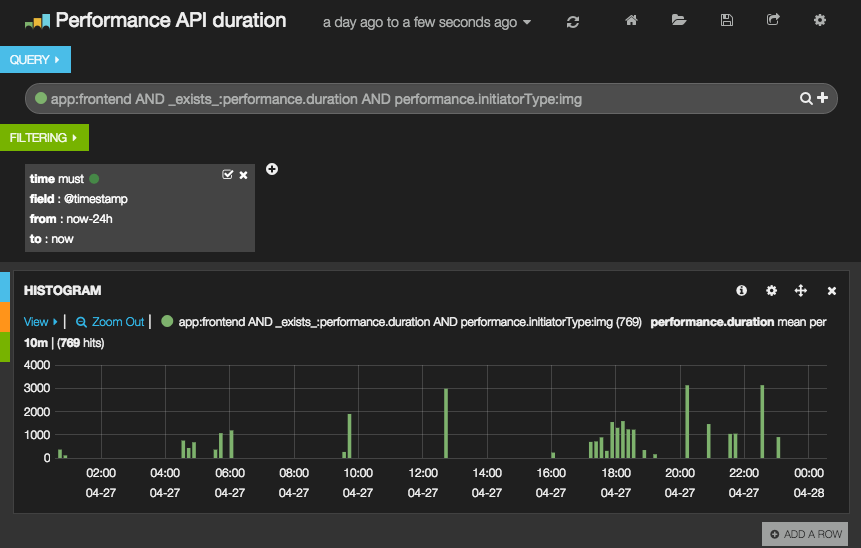
\includegraphics[scale=0.5]{assets/elk.png}%
		\caption[DUMMY]%
		{A Kibana interfésze}%
		\label{fig:kibana-webinterface}
\end{figure}

\Aref{fig:kibana-webinterface} ábrán látható a Kibana interfésze, ez egy webes alkalmazás, amelyben adhoc és állandó irányítópulton lehet vizsgálni az adatokat. A rendszer képes valós időben is megjeleníteni adatokat és az ElasticSearch mögött álló Lucene rendszernek köszönhetően a lekérdezéshetőség bő arzénálja áll rendelkezésre az a riportok tőkéletesítésére.

\section{Alkalmazás hibák\\}
A naplózással a hibák könnyen észrevehetővé és később visszakereshető válnak, azonban a következőkre nem nyújt megoldást:\\
\begin{itemize}
\item hibák rögzítése a jegykezelő (issue kezelő) rendszerben
\item egy hiba csak egyszer kerüljön rögzítésre
\item automatikus értesítés a hibáról
\item a hibaszázalék vizualizálása komponensenként
\end{itemize}

Természetesen egy alkalmazás hiba monitorozó rendszer nélkül is működhet jól, azonban előfordulhat, hogy nagy mennyiségű hibánál a naplógyűjtő rendszerben átsiklanak problémák felett vagy egyszerűen elfelejtésre kerülnek, mert a hibák megszokottá válnak ezért nem kezelik őket a megfelelő prioritással. A másik probléma lehet amikor a hibajelentést közvetlenül a jegykezelő rendszerbe kötik be. Ez miért lehet probléma? Egy nagy felhasználóbázissal rendelkező rendszernél, ha a hiba csak a felhasználók néhány százalékánál fordul elő, akkor is szükségtelenül nagy mennyiségű jegy keletkezést fogja előidézni.\\
\hfill\\
Az alkalmazás hiba monitorozás leginkább a nem webes alkalmazásoknál (mobil és asztali) terjedt el az utóbbi időben, ugyanis ezeknél a rendszereknél a naplók nem, vagy csak nehezen gyűjthetők valós időben.\\
\hfill\\
Legelterjedtebb alkalmazások:
\begin{itemize}
\item Sentry - \url{http://getsentry.com}
\item Exceptional - \url{http://www.exceptional.io/}
\item Bugsense - \url{http://www.bugsense.com/}
\end{itemize}

\begin{figure}[ht]
	\centering
		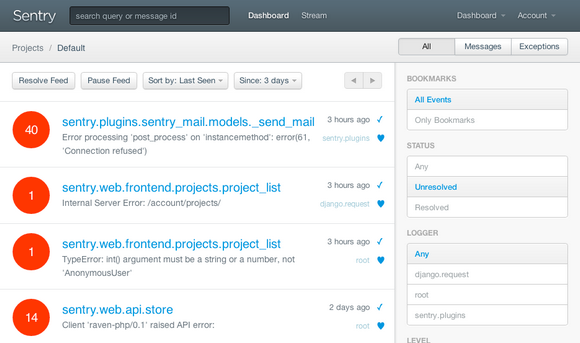
\includegraphics[scale=1]{assets/sentry.png}%
		\caption[DUMMY]%
		{A Sentry interfésze}%
		\label{fig:sentry}
\end{figure}

\section{Monitorozás}
A monitorozás a naplózás egy része, viszont míg a naplózást alapvetően öndiagnosztiként került bemutatásra \aref{sect:logging} pontban, ezért fontos kiemelni, hogy a monitorozás külső diagnosztikát jelent.\\
Olyan értelemben külső, hogy az alkalmazás működését bizonyos időközönként ellenőrzik. Ez jelentheti a másodpercenkénti többszöri vizsgálatát is annak, hogy működik-e a szoftver, a válaszidő mérése vagy akár biztonsághoz köthető mérések is lehet végezni. Általában a külső forrásból érkező ellenőrzések eredményei is a naplózó rendszerbe kerülnek bele és az alkalmazás belső naplóbejegyzéseivel együtt kerülnek elemzésre ezáltal próbálva meg rekonstruálni a felhasználók által érzékelt teljesítményt.

\section{Integráció\\}
\label{section:service_integration}
A fejezetben említett szolgáltatások, szoftverek (alkalmazás hiba monitorozó, naplógyűjtő, chat) használatával a fejlesztők, adminisztrátorok jobban megismerhetik saját alkalmazásaikat, azonban ennyi felület, különböző eszköz, aggregálatlan értesítés nyomon követése szinte már lehetetlen, ezért a legtöbb szervezet próbálja ezeket az eszközöket egymásba integrálni.
\begin{figure}[ht]
	\centering
		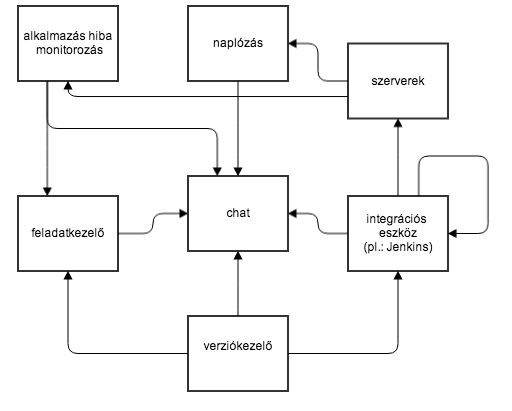
\includegraphics[scale=1.0]{assets/integrated_services.png}%
		\caption[DUMMY]%
		{A szolgáltatások egy lehetséges integrálása}%
		\label{fig:integrated-services}
\end{figure}
\Aref{fig:integrated-services} ábrán látható a szolgáltatások egy lehetséges integrációja. Első ránézésre az ábra bonyolultnak és összetettnek tűnhet, mert sok különböző egység közötti összeköttetés megvalósítását igényli, emellett a részegységeknek valós időben kell kommunikálniuk, ismerniük kell a sorrendet, és képeseknek kell lenniük egymás üzeneteinek megértésére.\\
Ezeknek az igénynek a kielégítésére minden részegység azt tudja, hogy kit kell neki értesítenie; az értesítések pedig ún. \emph{webhook} (\cite{web_hook}) használatával történnek, amely egy egyszerű HTTP kérés, ezáltal valós időben történhet meg az következő részegység értesítése.\\
Viszont hogyan képesek megérteni egymás üzeneteit a részegységek?\\
Erre sajnos nincs sztenderd specifikáció, azonban szinte minden említett eszköz nyílt forrású és széles körben elterjedt, ezért egymás üzeneteinek feldolgozása, megértése már megoldott beépülő modulok használatával.\\

\Aref{fig:integrated-services} ábrán felrajzolt folyamatnak az első szintje az amikor a kód bekerül a verziókezelőbe, amely össze van kapcsolva a feladatkezelővel, ahol akár a kapcsolódó jegy lezárásra is kerülhet a kód mellé csatolt üzenet szövege (\nomenclature{commit message}{TODO}) alapján, majd a chaten keresztül értesülhetnek a csapat tagjai, a projektmenedzser vagy az adott szervezeten belül bárki, aki érintett lehet az adott funkció, szolgáltatás fejlesztésében.\\
A verziókezelő másik kapcsolata az integrációs eszközzel van, amely lefuttatja az előre definiált ellenőrző, tesztelési és riportálási feladatokat, amelyek garantálják, hogy az új kódsorok megfelelnek a céges előírásoknak, nem okoznak problémát az alkalmazás futtatásában; a folyamat végén értesítést küldhet a közös chatbe az integráció sikerességéről, hiba esetén értesítheti a megfelelő személyeket, ugyanis a hiba kijavításáig senki tud hibamentes kódot beküldeni az integrációs folyamatba, ezért ennek az értesítésnek a legmagasabb prioritással kell megtörténnie. Az integrációs folyamat kimenete lehetséges, hogy újabb integrációs folyamat bemenete lesz; ez olyankor fordulhat elő, amikor az alkalmazás egyik ága egy másik ágba kerül beolvasztásra. Ez történhet például a fejlesztői ág tesztelői ágba való automatikus vagy félautomatikus olvasztásakor, vagy a minőségbiztosítási csapat (\nomenclature{QA team}{TODO}) tesztelői ág jóváhagyásaként a produkciós ágba való olvasztáskor.\\
\hfill\\
\Aref{fig:integrated-services} ábrán továbbhaladva az integrációs eszköz után az alkalmazás a felhasználói elfogadási szerverre (user acceptance test server) vagy előnézeti (staging, preview) szerverre kerül, amely egy homokozószerű, zárt, a produkciós szerverrel megegyező architektúrájú környezetben nyújt lehetőséget az alkalmazás tesztelésére. Majd ezután kerülhet ki a produkciós szerverre. Mind a felhasználói elfogadási, az előnézeti és a produkciós szerverek hibáit már naplózni kell illetve az ezeken futó alkalmazásokét is; hiba esetén pedig értesíteni kell (a chaten keresztül) a hibát okozó komponens, vagy az alkalmazás hibás részéért felelős személyt, csapatot (ideális esetben, ha a hibából a hiba pontos helye is megállapítható akkor a verziókezelő rendszer segítségével akár a hibás kódsort beküldő személy is értesíthető). A felelősök a hibáról hibajegyet készíthetnek a feladatkezelőbe, majd a fejlesztőcsapatok javítva a hibát a kódot beküldik a verziókezelőbe és a folyamat újraindul.\\
\hfill\\
Fontos felhívni a figyelmet, hogy \aref{fig:integrated-services} ábrán rendkívül komoly hangsúlyt kapott a chat rendszer, természeten nem kötelező csetet használni, azonban a valós idejű értesítésekre illetve a reakcióidő csökkentése érdekében mindenképpen ajánlott. Továbbá az ábrán nem szerepel, de a cset alapú notifikálás mellett érdemes egyéb értesítési formákat is használni, mint például az email, vagy magas prioritású hibáknál (alkalmazásleállás) érdemes lehet megfontolni az sms, okostelefonos valós idejű üzenet (\nomenclature{Push Notification}{TODO}), esetleg csipogó használata is.

\subsection{Automatizálás}
\label{subsec:automating}
Ha egy szervezet úgy dönt, hogy a folyamatait mélyen egymásba integrálja akkor rövid találkozni fog a következő problémákkal:
\begin{description}
\item[Rendszer-automatizáció lépései]\hfill\\
Hiába automatizált a folyamat, ha az egy-egy pontról történő elindítás/újraindítás nem lehetséges, bárhonnan, bármikor akkor rengeteg plusz munkát igényel a megelőző (és már korábban sikeresen végrehajtott) lépések újbóli végrehajtása.\\
Ilyen probléma lehet az integrációs rendszer elindítása a kód egy pillanatnyi állapotától kód beküldés nélkül, amelyet gyakran nem tesznek lehetővé, pedig a kód életében sokszor előfordul, hogy az integráció egy kivülálló ok (instabil hálózati kapcsolat, a rendszer általános leterheltsége) sikertelen státuszba és újra kell indítani új kód beküldése nélkül.

\item[Távoli irányítás]\hfill\\
Lehet, hogy egy asztali számítógépen könnyen elvégezhető a produkciós rendszerben egy verzióváltás, de miért ne lehetne ezt megtenni bármilyen más eszközről, akár okostelefonról keresztül?

\item[Kommunikáció külső eszközök használatakor]\hfill\\
Ha egy üzenet érkezik (például alkalmazás újraindítás szükségességéről), akkor a csapat tagjainak meg kell beszélniük, hogy ki javítja meg a problémát.
\end{description}

Ezekre a problémákra egyszerű megoldásként javallott a robotok alkalmazása, amely képesek emulálni a felesleges lépéseket a folyamatokban; egyszerű felületet, hozzáférést nyújtanak akár okostelefonok számára is illetve könnyen illeszkednek a kommunikációba.

\paragraph{Hubot - http://hubot.github.com/} A GitHub ingyenesen elérhető chat robotja \aref{subsec:automating} alfejezetben említett problémákra próbál egyszerű és univerzális megoldást nyújtani. Képes együttműködni \aref{table:chat-system-compare} táblázatban található összes alkalmazással és mindezek mellett észrevétlenül integrálódik a feladatkezelő rendszerekkel, a hibagyűjtő alkalmazásokkal. Továbbá az elérhető dokumentációknak, a nagy mennyiségű közösségi támogatásnak és a széles körű használatának köszönhetően bárki készíthet hozzá egyéni kiegészítőket melyekkel a saját belső rendszerekkel is könnyen integrálódhat. A kiegészítők hivatalos gyűjteménye a \url{https://hubot-script-catalog.herokuapp.com/} címen érhető el.\\
\hfill\\
Fontos megjegyezni, hogy egy chat robottal nem a chat kerül automatizálásra, hanem a rendszert felépítő szolgáltatások.\\
\hfill\\
De akkor miért érdemes robottal automatizálni, miért nem más rendszerrel teszik mindezt? A válasz két részből áll, az egyik ha a szervezet rendelkezik cset rendszerrel akkor egy újabb rendszer megismerése problémás lehet. A másik ok pedig a kontextus váltások minimalizálása, azaz ha a felelős személyeknek elég a chaten egy megfelelő parancsot kiadni (például ahelyett, hogy belépnek a feladatkezelő rendszerbe, ahol átállítják a megfelelő állapotra a hibajegyet), akkor időt spórolhatnák és mindemellett a chaten keresztül a csapat többi tagja is látja, hogy éppen ki mit csinál, vagy akár később a chat naplóból is visszaellenőrizhető a végrehajtott lépések sorozata. A chat alapú működésről bővebben \aref{chapter:chatops}. fejezet foglalkozik.
